\documentclass{article}
\usepackage[a4paper, total={6in,9in}]{geometry}
\usepackage{fancyhdr}
\usepackage{graphicx}

\begin{document}
\pagestyle{fancy}
\fancyhead[L]{CS1010 -- Intro to Information Technology}
\fancyhead[R]{Final Project}

\section{Wordle}
\hspace{\parindent}For this project, you will be recreating the popular game \emph{Wordle}! For those who haven't played, \emph{Wordle} is a word game in which the player has a secret 5-letter word. After each guess, the user is given information regarding how each letter of their guess fits into the secret word (i.e. whether or not each letter is in the word and/or in the correct spot).

\vspace{0.5cm}

\begin{figure}[h!]
    \centering
    \fbox{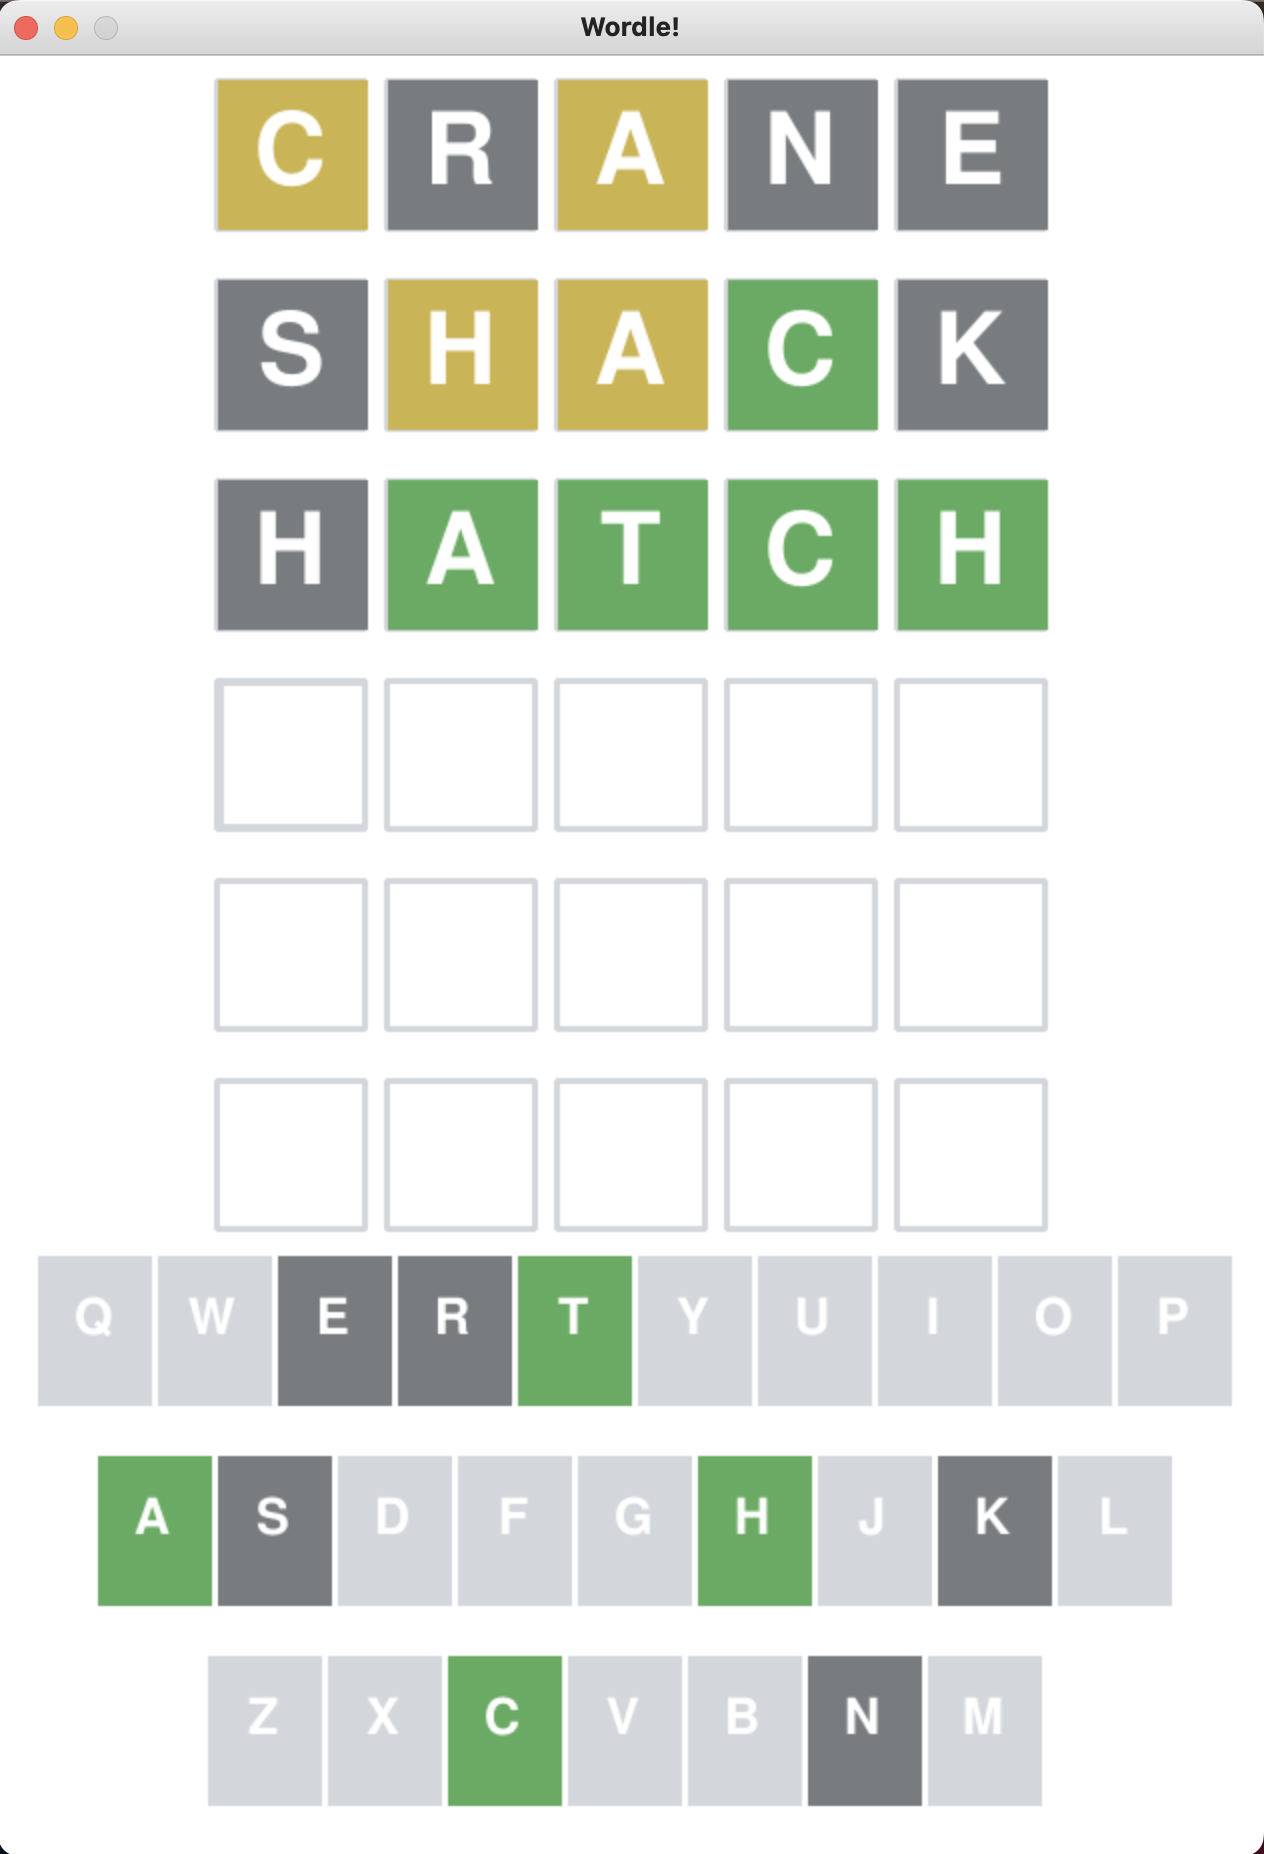
\includegraphics[width=0.6\textwidth]{wordle.png}}
    \caption{Example for the secret word \emph{``CRANE"}.}
\end{figure}

\vspace{1cm}

Of the code provided, the only file that you are allowed to modify is \emph{wordle\_starter.py}, which contains starter code for the project. To start the program, simply run \emph{wordle\_starter.py}. Your job will be to program the logic behind Wordle, which requires your implementation of three methods, outlined in the following subsections.

\subsection{Part 1: Initialize the Game (10 pts.)}
\hspace{\parindent} To select a secret word and to determine whether or not a guess is valid, \emph{Wordle} uses a long list of ``valid words." The file \emph{words.txt} (provided for you) contains over two thousand valid 5-letter words, one per line. Your job is to implement the \emph{init\_game()} method, which accepts the file path  (of type \emph{string}) as input, and outputs a \underline{randomly selected} secret word. Implement the following inside of the \emph{init\_game()} method:

\begin{enumerate}
\itemsep0em 
\item{Randomly select the secret word}
\item{Return the secret word.}
\end{enumerate}

\subsection{Part 2: The Game Loop (10 pts)}
\hspace{\parindent}Now that we have a word selected, we must begin accepting user input in what is called the ``Game Loop''. This is a loop that will continue until the game is over.

\begin{enumerate}
\itemsep0em 
\item{Keep track of how many times the user guesses}
\item{Check that the player's guess is exactly 5 letters long.}
\item If the guess is 5 letters long, then use the eval\_guess function
\item Return the number of guesses at the end of the function 
\end{enumerate}

\subsection{Part 3: Evaluate a Guess (20 pts)}
\hspace{\parindent}Now that you have verified that a guess is valid, we need to evaluate the guess and tell the user how they did. In \emph{Wordle}, each letter in the guess is evaluated to be: \emph{a)} correct letter in the correct position, \emph{b)} correct letter in the wrong position, or \emph{c)} incorrect letter. Your job is to implement the \emph{eval\_guess()} method, which accepts the secret word and the user's guess as input, and outputs a letter-by-letter evaluation of the guess. Implement the following inside of the \emph{eval\_guess()} method:

\begin{enumerate}
\itemsep0em 
\item{Loop through each letter of the guess and determine how it should be evaluated, based on the secret word.}
\item{Construct an output string that contains each correct letter in the correct position, a `$\ast$' for each correct letter in the incorrect position, and a `\#' for each incorrect letter. For example, if the secret word is \emph{``CRANE"} and the user guesses \emph{``LEARN"}, the evaluation should be the string \emph{``\#$\ast$A$\ast \ast$"}.}
\item{Return the evaluation string, as constructed in the previous step.}
\end{enumerate}

\subsection{Code Submission}
Congratulations -- you just recreated the game \emph{Wordle}! The only code that you must include in your submission is the \emph{wordle\_starter.py} file.

\newpage
\subsection{Questions (10 pts)}
\subsubsection{For Part 1, how did you ensure that you selected a random word? (2 pts)}
\vspace{2in}

\subsubsection{For Part 2, how did you ensure the guess was a valid guess? What did you do if it wasn't valid? (3 pts)}
\vspace{2in}

\subsubsection{For Part 3, what challenges did you face when handling this portion of the project? How did you check that you were correctly evaluating the guess? (5 pts)}
\vspace{2in}

\end{document}